\documentclass[border=2mm]{standalone}
\usepackage{tikz}
\usetikzlibrary{calc,patterns,angles,quotes}
\begin{document}
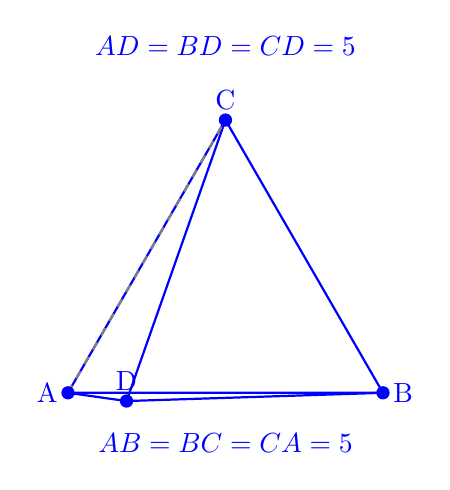
\begin{tikzpicture}[scale=0.8,blue,thick]
\coordinate (A) at (0,0,0);
\coordinate (B) at (5,0,0);
\coordinate (C) at (2.5,4.33,0);
\coordinate (D) at (2.5,1.44,4.08);

\draw (A) -- (B) -- (C) -- cycle;
\draw (A) -- (D);
\draw (B) -- (D);
\draw (C) -- (D);
\draw[dashed,gray] (A) -- (C);

\fill[blue] (A) circle (3pt);
\fill[blue] (B) circle (3pt);
\fill[blue] (C) circle (3pt);
\fill[blue] (D) circle (3pt);

\node[left] at (A) {A};
\node[right] at (B) {B};
\node[above] at (C) {C};
\node[above] at (D) {D};

\node at (2.5,-0.8) {$AB=BC=CA=5$};
\node at (2.5,5.5) {$AD=BD=CD=5$};
\end{tikzpicture}
\end{document}